\begin{boxK}
با شکسته‌شدن الگوریتم
\grayBox{\lr{DES}}
، 
در سال ۲۰۰۱ 
الگوریتم
\grayBox{\lr{AES}}
به عنوان استاندارد رمزنگاری انتخاب شد.
در مورد نحوه این انتخاب ، ساختار و چگونگی کارکرد این الگوریتم تحقیق کنید.
\end{boxK}

\begin{boxL}
در استاندارد رمزنگاری پیشرفته کامل ، 
\grayBox{\lr{AES - Advanced Encryption Standard}}
یک استاندارد رمزنگاری داده تایید شده توسط موسسه ملی استانداردها و فناوری ایالات متحده به عنوان جایگزینی برای الگوریتم
\grayBox{\lr{DES}}
خواهد بود.

در ژانویه ۱۹۹۷ 
\grayBox{\lr{NIST}}
یک درخواست عمومی برای ایجاد یک الگوریتم برای جایگزینی 
الگوریتم 
\grayBox{\lr{DES}}
ایجاد کرد.

۱۵ 
کاندیدا از 
۱۲ 
کشور
برای این درخواست الگوریتم‌های خود را ارائه کردند.

 
 در اکتابر ۲۰۰۰
دو
رمزنگار بلژیکی  ،
ریژمان و دیمن
الگوریتمشان به عنوان یک استاندارد جدید مورد پذیرش قرار گرفت.

اداره ملی استانداردها ،
\grayBox{\lr{NIST}}
انتظار داشت که
\grayBox{\lr{DES}}
در سخت‌افزار با هدف خاص پیاده‌سازی شود و از این‌رو به اجرای کارآمد آن در نرم‌افزار توجه چندانی نکرده بود.

به عنوان مثال استفاده از ریزپردازنده‌های همه‌منظوره .

در نتیجه 
\grayBox{\lr{DES}}
نتوانست از پیشرفت سریع ریزپردازنده‌ها که در دو دهه آخر قرن بیستم رخ داد ، استفاده کند.

از سوی دیگر ، مشخصات 
\grayBox{\lr{AES}}
بر پیاده‌سازی سخت‌افزاری و نرم‌افزاری به طور مساوی تاکید داشت.

این امر تا حدی نیازهای کارت‌های هوشمند و سایر تجهیزات نقطه‌فروشی را که معمولاً قابلیت‌های محاسباتی بسیار محدودی دارند، شناسایی کرد.

اما مهم‌تر شناخت نیازهای رو‌به‌رشد اینترنت و تجارت الکترونیک بود.

بر اساس تجربه آن‌ها با
\grayBox{\lr{DES}} ،
که در آن پیشرفت‌ها در محاسبات به سادگی بر ضریب کارکلید کد ۵۶ ثابت فائق آمد.

همچنین سازمان ملی استانداردهای آمریکا یا همان

خواستار این شد که الگوریتم بتواند در صورت لزوم طول کلید را افزایش دهد.

\grayBox{\lr{Rijndael}}
ثابت کرد که
کلیدها
هم به اندازه کافی 
کوچک است که بتوان بر روی کارت‌های هوشمند پیاده‌سازی کرد و هم به اندازه کافی انعطاف پذیر است که طول کلیدهای طولانی تری را ایجاد کند.
\end{boxL}

\begin{figure}[h]
    \centering
    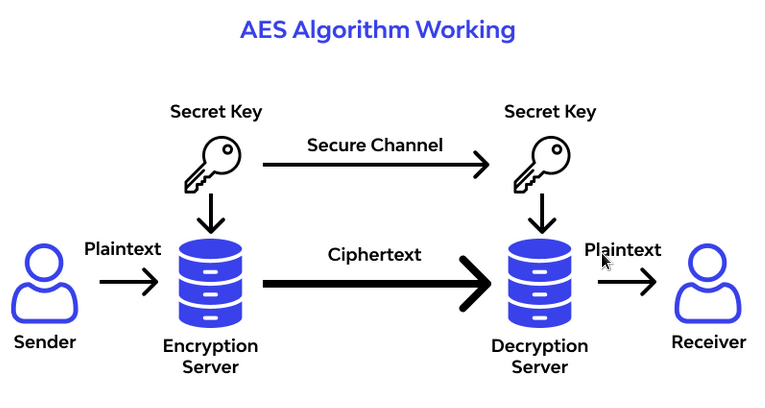
\includegraphics
    [width = 0.8\textwidth]
    {HW3/images/AES_Sch.png}
    \caption{رویه کلی الگوریتم}
    \label{fig:my_label}
\end{figure}

\begin{boxL}
    استاندارد رمزنگاری پیشرفته یا همان
    \grayBox{\lr{AES}}
    ، یک الگوریتم رمزنگاری بلوکی ۱۲۸ بیتی متقارن است
    که داده ورودی را پس از انجام عملیات رمزنگاری یا
    \grayBox{\lr{Encryption}}
    تبدیل به یک کلید رمز می‌کند.

    کلمه متقارن در اینجا به این معنی است که یک
    \grayBox{\lr{Secret Key}}
    مشترک برای رمزنگاری و رمزگشایی داده استفاده‌می‌شود و باید در هر دو سمت یک رمز مشترک وارد شود.

    به عبارت ساده‌تر ، 
    \grayBox{\lr{AES}}
    یک بلوک رمزنگاری ۱۲۸ بیتی است که داده‌هایی با طول ۱۲۸ بیتی وارد آن می‌شوند و روی آن عملیات رمزنگاری را انجام می‌دهد که در اولین مرحله از رمزنگاری داده‌ها داخل یک آرایه قرار گیرند، سپس عملیات منطقی
    \grayBox{\lr{XOR}}
    است که روی هر ستون و کلید مربوطه اعمال می‌شود.

    سپس بسته به  طول رمزنهایی و ساختار آن مراحل بعدی به تعداد مشخصی تکرار می‌شوند که خروجی نهایی آن یک کلید برای دسترسی به اطلاعات رمزنگاری شده‌است.
\end{boxL}